\documentclass{paper}
\usepackage{graphics}
\usepackage{graphviz}
\usepackage{mathtools}
\begin{document}

\includegraphics[]{./SpecDecBot-Main.png}
\newline\newline
\begin{large}{an NLP dependant Clever Bot for Critical Decision Affirmation\newline\newline}\end{large}
\Large{\textbf{the Developers}}
\textit{,`by alphabetical order`:\newline}
Aly Shmahell, Alya Salman, Elias Soud\newline
Mohammad Shbani, Ruaa Sleiman, Sarah Ammar\newline\newline
\begin{Large}{\textbf{the Supervisor:}}\end{Large}
Dr. Hasan Ahmad\newline
\newline
\textbf{\textit{a $ 4^{th} $ year Project for the Dep. of Computer and Automatic Control Engineering @ Tishreen University}}\newline\newline
\begin{center}
Documentation \textit{v(0.1)}\newline
$ 26^{th} $ of November $ 2015 $\newline
\end{center}
\newpage
\begin{huge}{\textbf{License\newline\newline}}\end{huge}
\begin{large}
Copyright 2015 The SpecDecBot Project (Aly Shmahell, Alya Salman, Elias Soud, Mohammad Shbani, Ruaa Sleiman, Sarah Ammar). All rights reserved.

Redistribution and use in source (Graphml,svg,tex and so forth) and 'compiled' forms (HTML, PDF, PNG, JPG, PostScript, RTF and so forth) with or without modification, are permitted provided that the following conditions are met:

Redistributions of source code (Graphml,svg,tex and other formats) must retain the above copyright notice, this list of conditions and the following disclaimer as the first lines of this file unmodified.

Redistributions in compiled form (HTML, PDF, PNG, JPG, PostScript, RTF and other formats) must reproduce the above copyright notice, this list of conditions and the following disclaimer in the documentation and/or other materials provided with the distribution.

THIS DOCUMENTATION IS PROVIDED BY THE SPECDECBOT PROJECT "AS IS" AND ANY EXPRESS OR IMPLIED WARRANTIES, INCLUDING, BUT NOT LIMITED TO, THE IMPLIED WARRANTIES OF MERCHANTABILITY AND FITNESS FOR A PARTICULAR PURPOSE ARE DISCLAIMED. IN NO EVENT SHALL THE SPECDECBOT PROJECT BE LIABLE FOR ANY DIRECT, INDIRECT, INCIDENTAL, SPECIAL, EXEMPLARY, OR CONSEQUENTIAL DAMAGES (INCLUDING, BUT NOT LIMITED TO, PROCUREMENT OF SUBSTITUTE GOODS OR SERVICES; LOSS OF USE, DATA, OR PROFITS; OR BUSINESS INTERRUPTION) HOWEVER CAUSED AND ON ANY THEORY OF LIABILITY, WHETHER IN CONTRACT, STRICT LIABILITY, OR TORT (INCLUDING NEGLIGENCE OR OTHERWISE) ARISING IN ANY WAY OUT OF THE USE OF THIS DOCUMENTATION, EVEN IF ADVISED OF THE POSSIBILITY OF SUCH DAMAGE.
\end{large}
\newpage
\begin{huge}{\textbf{Preface\newline}}\end{huge}

\textit{`I Think Therefor I Am`,} is the standard when defining human intelligence, and by far any intelligence. However, so far the intelligence we've encountered doesn't only think, but also feels, Something that has guided our passion and exploded in various forms of creativity.\newline\newline
but with great passion comes risk, the risk to make rash decisions, rookie mistakes. pulling all-nighters at the office passionately trying to maximize the stock profits, or all those hours standing in the lab experimenting with life-saving medicinals and waiting for results, all that exhaustion puts your decisions at jeopardy.\newline\newline
Human Error, is by far the most fatal, because we trust our decision so much we're willing to stake everything on them, but what happens when you're under pressure but can't perform optimally?
\newline
You need something both capable of carrying your tasks and understanding them in layman terms, and something that is cryptographically secure.\newline\newline
For  that we present you dear user with SpecDecBot, an Artificial Agent capable of comprehending binary work-related questions using Natural Language Processing techniques and running them against specialty algorithms that perform optimally under all circumstances.
\newpage
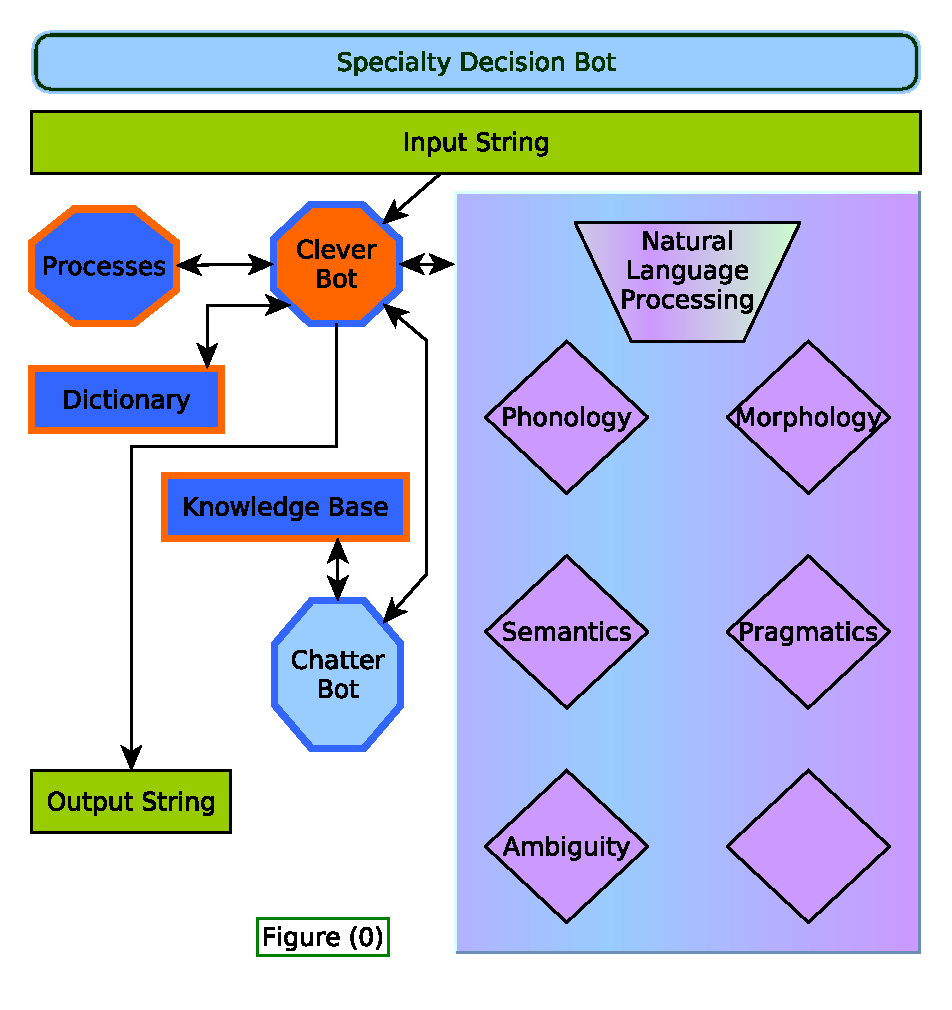
\includegraphics[]{./SpecDecBot-Diagram0.pdf}
\newpage
\begin{huge}{\textbf{Introduction}}\end{huge}\newline\newline
As illustrated in figure (0), the Project has an object-oriented work-flow, which goes as follows :\newline\newline
1)- an Input string is provided to a clever-bot.\newline
2)- the clever-bot utilizes an NLP class to mine a dictionary and create a semantic tree for the input string.\newline
3)- if the tree is successfully created, the bot uses the dictionary to link the tree with algorithms from the processes library.\newline
4)- the algorithms use input from the semantic tree and answer the intended question in a binary matter.\newline
5)- the bot uses the binary answer the NLP class, and the Dictionary to create a second semantic tree for an answer.\newline
6)- the bot converts the answer's semantic tree to an output-string.\newline
7)- in case the first semantic tree (the question's) is not created for reasons like "incomplete semantic tree, faulty input, or illogical input" or if the tree is incoherent, the clever-bot communicates with the user to try and correct the Error.\newline\newline
\textit{notice} : the Clever-Bot performs Semantic-Tree operations, String-Conversion and Algorithm-Linking operations.\newline
however, it can also communicate with the user in an interactive manner using suggestions from an embedded Chatter-Bot.
\end{document}